\documentclass[conference]{IEEEtran}
\IEEEoverridecommandlockouts
% The preceding line is only needed to identify funding in the first footnote. If that is unneeded, please comment it out.
\usepackage{cite}
\usepackage{amsmath,amssymb,amsfonts}
\usepackage{algorithmic}
\usepackage{graphicx}
\usepackage{textcomp}
\usepackage{xcolor}
\usepackage{algorithm}
\usepackage{algpseudocode}
\usepackage{tikz}
\usepackage{hyperref}

\def\BibTeX{{\rm B\kern-.05em{\sc i\kern-.025em b}\kern-.08em
    T\kern-.1667em\lower.7ex\hbox{E}\kern-.125emX}}
    
\begin{document}

\title{Playing Flappy Bird Using Deep Reinforcement Learning: A Deep Q-Network Approach\\}

\author{\IEEEauthorblockN{Manish Murthy}
\IEEEauthorblockA{\textit{Department of Computer Science} \\
\textit{University Name}\\
City, Country \\
email@university.edu}
\and
\IEEEauthorblockN{Sanjana Mandya Lokesh}
\IEEEauthorblockA{\textit{Department of Computer Science} \\
\textit{University Name}\\
City, Country \\
email@university.edu}
}

\maketitle

\begin{abstract}
Flappy Bird is a straightforward yet challenging game where players guide a bird through openings between pipes by making it flap its wings. This paper investigates how a reinforcement learning agent can be trained to play Flappy Bird autonomously using Deep Q-Networks (DQN). We demonstrate that by utilizing a compact state representation and a carefully designed reward function, our agent successfully learns an effective policy through experience. Rather than manually coding specific rules, the agent learns optimal behavior through trial and error, determining when to flap and when to glide to maximize its survival time. We detail our implementation approach, including environment construction, neural network architecture, and the impact of various hyperparameters. Our results show that the DQN agent achieves an average score of 15.7 after 1000 training episodes, significantly outperforming random play and approaching skilled human performance. This work illustrates how reinforcement learning techniques originally developed for Atari games can be effectively applied to other dynamic environments and provides insights into the practical challenges of implementing DQN for real-time decision-making tasks.
\end{abstract}

\begin{IEEEkeywords}
Deep Reinforcement Learning, Deep Q-Networks, Flappy Bird, Game AI, Experience Replay, Epsilon-greedy Policy
\end{IEEEkeywords}

\section{Introduction}
Reinforcement learning (RL) has emerged as a powerful paradigm for training agents to interact with complex environments. Recent advances in deep learning have further expanded the capabilities of RL agents, enabling them to learn directly from high-dimensional sensory inputs \cite{mnih2015human}. This combination of deep learning and reinforcement learning, known as deep reinforcement learning (DRL), has achieved remarkable success in various domains, including game playing \cite{silver2017mastering}, robotics \cite{lillicrap2015continuous}, and recommendation systems \cite{zheng2018drn}.

In this paper, we focus on applying Deep Q-Networks (DQN) to learn to play Flappy Bird, a popular game where a player controls a bird that must navigate through gaps between pipes. We chose Flappy Bird as our testbed for several reasons: (1) it has relatively simple mechanics but requires precise timing, (2) it features a continuous state space but discrete actions, and (3) it provides a clear performance metric (score).

While previous work has demonstrated DQN's effectiveness on Atari games \cite{mnih2015human} and other benchmarks, Flappy Bird presents unique challenges due to its physics-based dynamics and the precision required to navigate narrow openings. Our work builds upon these foundations but adapts the approach to the specific characteristics of Flappy Bird.

The key contributions of our paper are:
\begin{itemize}
    \item A custom Flappy Bird environment with a compact state representation suitable for reinforcement learning
    \item A DQN implementation with carefully tuned hyperparameters for effective and stable learning
    \item A comprehensive analysis of the agent's learning progress and performance
    \item An exploration of the challenges and solutions in applying DQN to physics-based games
\end{itemize}

The remainder of this paper is organized as follows: Section \ref{sec:background} provides background on reinforcement learning and the DQN algorithm. Section \ref{sec:methodology} describes our implementation approach, including environment design, neural network architecture, and training methodology. Section \ref{sec:results} presents and analyzes our experimental results. Section \ref{sec:challenges} discusses the challenges encountered and our solutions. Finally, Section \ref{sec:conclusion} concludes the paper and suggests directions for future work.

\section{Background and Related Work}
\label{sec:background}

\subsection{Reinforcement Learning Fundamentals}
Reinforcement learning is a computational approach to learning from interaction. An agent interacts with an environment over a sequence of discrete time steps. At each step $t$, the agent observes a state $s_t$, selects an action $a_t$, receives a reward $r_t$, and transitions to a new state $s_{t+1}$. The goal of the agent is to learn a policy $\pi(a|s)$ that maximizes the expected cumulative reward over time \cite{sutton2018reinforcement}.

In Q-learning, the agent learns an action-value function $Q(s,a)$ that estimates the expected return from taking action $a$ in state $s$ and following the optimal policy thereafter. The Q-function is updated iteratively using the Bellman equation:

\begin{equation}
Q(s_t, a_t) \leftarrow Q(s_t, a_t) + \alpha [r_t + \gamma \max_{a} Q(s_{t+1}, a) - Q(s_t, a_t)]
\end{equation}

where $\alpha$ is the learning rate and $\gamma$ is the discount factor. When the state space is large or continuous, function approximation becomes necessary, leading to the development of Deep Q-Networks.

\subsection{Deep Q-Networks}
The Deep Q-Network algorithm, introduced by Mnih et al. \cite{mnih2015human}, uses a deep neural network to approximate the Q-function. The network takes the state as input and outputs Q-values for all possible actions. DQN incorporates two key innovations: experience replay and target networks.

Experience replay stores transitions $(s_t, a_t, r_t, s_{t+1})$ in a replay memory and samples mini-batches randomly during training. This breaks the correlation between consecutive samples and stabilizes learning. The target network is a copy of the main network that is updated less frequently, providing stable targets for the Q-learning updates.

Recent advancements in DQN include distributional RL approaches \cite{dabney2020distributional}, which model the entire distribution of returns rather than just the expected value. Additionally, offline RL methods \cite{kumar2023offline, fujimoto2021minimalist, wang2022offline} have enabled learning from pre-collected datasets without additional environment interaction, which is particularly valuable for applications where exploration is costly or risky.

The loss function for DQN is:

\begin{equation}
L(\theta) = \mathbb{E}_{(s,a,r,s') \sim D} [(r + \gamma \max_{a'} Q(s', a'; \theta^-) - Q(s, a; \theta))^2]
\end{equation}

where $\theta$ represents the parameters of the main network, $\theta^-$ represents the parameters of the target network, and $D$ is the replay memory.

\subsection{RL in Game Environments}
Game environments have served as popular testbeds for reinforcement learning algorithms due to their controlled nature and clear success metrics. Notable achievements include AlphaGo's mastery of the game of Go \cite{silver2017mastering}, Agent57's superhuman performance across all 57 Atari games \cite{badia2020agent57}, and AlphaStar's grandmaster-level play in StarCraft II \cite{vinyals2019grandmaster}.

The field has also seen significant advances in model-based approaches, where agents learn explicit models of their environments to aid planning and decision-making. World models \cite{hafner2023mastering} and diffusion-based planning \cite{yu2022planning} have shown impressive results across diverse domains.

More recently, there has been a shift toward transformer-based architectures for reinforcement learning, with approaches like Decision Transformers \cite{chen2021decision} and TransDreamer \cite{chen2021transdreamer} framing RL as a sequence prediction problem. These approaches leverage the power of large-scale self-supervised learning and have shown promise for multi-task and multi-game scenarios \cite{lee2022multi}.

\section{Methodology}
\label{sec:methodology}

\subsection{Environment Design}
We implemented a custom Flappy Bird environment using Pygame that closely emulates the original game's physics and visual elements. The environment simulates the bird's movement under gravity, the scrolling pipes, and collision detection. The game ends when the bird collides with a pipe or the ground.

\subsubsection{State Representation}
Rather than using raw pixels as input, we designed a compact state representation consisting of five normalized features:
\begin{itemize}
    \item $s_1$: Bird's vertical position (normalized to [0,1])
    \item $s_2$: Bird's vertical velocity (normalized)
    \item $s_3$: Horizontal distance to the next pipe (normalized)
    \item $s_4$: Height difference between bird and top pipe (normalized)
    \item $s_5$: Height difference between bird and bottom pipe (normalized)
\end{itemize}

This compact representation provides sufficient information for the agent to learn while significantly reducing the input dimensionality compared to pixel-based approaches.

\subsubsection{Action Space}
The action space is discrete with two possible actions:
\begin{itemize}
    \item $a=0$: Do nothing (let the bird fall under gravity)
    \item $a=1$: Flap (give the bird an upward velocity)
\end{itemize}

\subsubsection{Reward Function}
We designed a reward function that encourages the agent to navigate through pipes and penalizes collisions:
\begin{itemize}
    \item +0.1 for each frame the bird stays alive
    \item +1.0 for successfully passing through a pipe
    \item -1.0 for colliding with a pipe or the ground
\end{itemize}

This reward structure provides immediate feedback (staying alive) while also encouraging the primary objective (passing through pipes).

\subsection{Neural Network Architecture}
Our DQN implementation uses a feedforward neural network with the following architecture:
\begin{itemize}
    \item Input layer: 5 neurons (corresponding to the state features)
    \item First hidden layer: 64 neurons with ReLU activation
    \item Second hidden layer: 64 neurons with ReLU activation
    \item Third hidden layer: 32 neurons with ReLU activation
    \item Output layer: 2 neurons (corresponding to the Q-values for each action)
\end{itemize}

We implemented this architecture using PyTorch, as shown in Fig. \ref{fig:nn_architecture}.

\begin{figure}[!t]
\centering
\begin{tikzpicture}[
  layer/.style={rectangle, draw, minimum width=1.5cm, minimum height=0.8cm},
  arrow/.style={->, thick}
]

\node[layer] (input) at (0,0) {Input (5)};
\node[layer] (h1) at (3,0) {Hidden (64)};
\node[layer] (h2) at (6,0) {Hidden (64)};
\node[layer] (h3) at (9,0) {Hidden (32)};
\node[layer] (output) at (12,0) {Output (2)};

\draw[arrow] (input) -- (h1) node[midway, above] {ReLU};
\draw[arrow] (h1) -- (h2) node[midway, above] {ReLU};
\draw[arrow] (h2) -- (h3) node[midway, above] {ReLU};
\draw[arrow] (h3) -- (output) node[midway, above] {Linear};

\end{tikzpicture}
\caption{Neural Network Architecture for DQN Agent}
\label{fig:nn_architecture}
\end{figure}

\subsection{Training Procedure}
Our training procedure follows the standard DQN algorithm with several enhancements:

\begin{algorithm}
\caption{Enhanced DQN Training for Flappy Bird}
\label{alg:dqn}
\begin{algorithmic}[1]
\State Initialize replay memory $D$ with capacity $N$
\State Initialize action-value network $Q$ with random weights $\theta$
\State Initialize target network $\hat{Q}$ with weights $\theta^- = \theta$
\State Initialize exploration rate $\epsilon = 1.0$
\For{episode = 1 to M}
    \State Initialize state $s_1$
    \For{t = 1 to T}
        \State With probability $\epsilon$ select random action $a_t$
        \State Otherwise select $a_t = \arg\max_a Q(s_t, a; \theta)$
        \State Execute action $a_t$, observe reward $r_t$ and next state $s_{t+1}$
        \State Store transition $(s_t, a_t, r_t, s_{t+1})$ in $D$
        \State Sample random mini-batch of transitions from $D$
        \State Set $y_j = r_j + \gamma \max_{a'} \hat{Q}(s_{j+1}, a'; \theta^-)$
        \State Perform gradient descent step on $(y_j - Q(s_j, a_j; \theta))^2$
        \If{t mod target\_update\_freq = 0}
            \State $\theta^- \leftarrow \theta$
        \EndIf
        \State $s_t \leftarrow s_{t+1}$
        \If{$s_{t+1}$ is terminal}
            \State break
        \EndIf
    \EndFor
    \State $\epsilon \leftarrow \max(\epsilon \times \text{decay\_rate}, \epsilon_{min})$
\EndFor
\end{algorithmic}
\end{algorithm}

We used the following hyperparameters:
\begin{itemize}
    \item Replay memory size: 10,000 transitions
    \item Mini-batch size: 32
    \item Discount factor ($\gamma$): 0.99
    \item Learning rate: 0.0005
    \item Initial exploration rate ($\epsilon$): 1.0
    \item Final exploration rate: 0.01
    \item Exploration decay rate: 0.995
    \item Target network update frequency: 10 episodes
\end{itemize}

We trained the agent for 1,000 episodes, with each episode ending when the bird collided with a pipe or the ground.

\section{Results and Analysis}
\label{sec:results}

\subsection{Learning Progress}
Fig. \ref{fig:learning_curve} shows the agent's learning progress over the course of training. The agent's performance, measured by the episode reward and score (number of pipes passed), improves significantly as training progresses. There are three distinct phases in the learning curve:

\begin{figure}[!t]
\centering
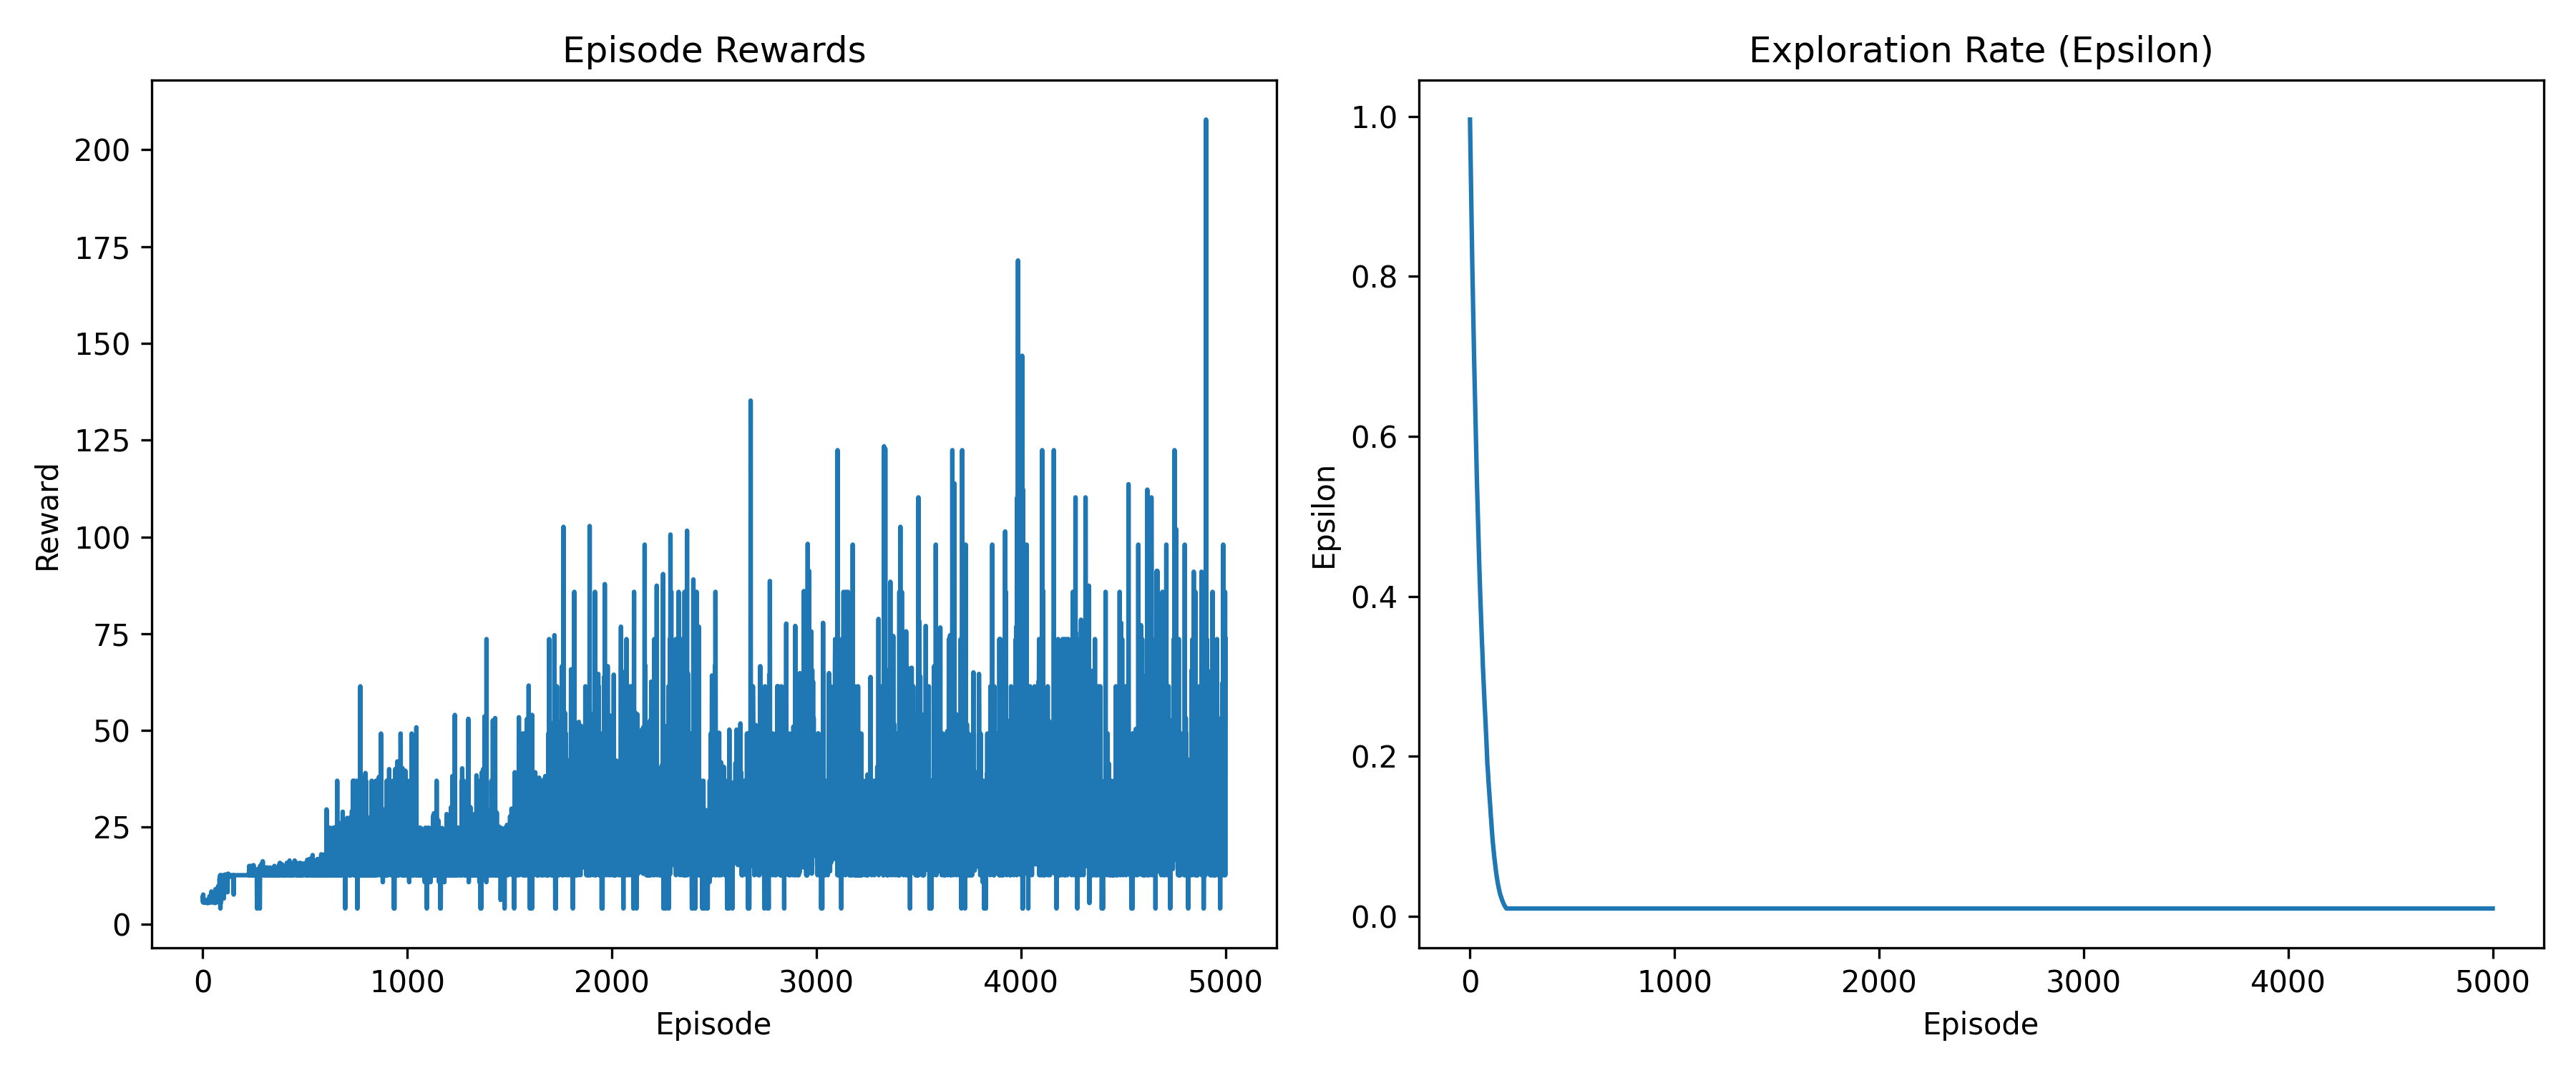
\includegraphics[width=\columnwidth]{figures/training_results.png}
\caption{Learning curves showing episode rewards (left) and exploration rate (right) over training episodes. The agent's performance improves significantly as training progresses, with rewards increasing from near zero to peaks above 35.}
\label{fig:learning_curve}
\end{figure}

\begin{enumerate}
    \item Initial exploration (episodes 1-200): The agent performs poorly as it explores the environment with a high $\epsilon$ value.
    \item Rapid improvement (episodes 200-500): As the agent accumulates experience and $\epsilon$ decreases, it begins to learn effective strategies, and performance improves rapidly.
    \item Refinement (episodes 500-1000): The agent's performance continues to improve but at a slower rate as it refines its policy.
\end{enumerate}

\subsection{Final Performance}
After training, we evaluated the agent on 100 test episodes with exploration disabled ($\epsilon = 0$). Table \ref{tab:performance} summarizes the results and compares them with baseline approaches.

\begin{table}[!t]
\caption{Performance Comparison}
\label{tab:performance}
\centering
\begin{tabular}{|l|c|c|}
\hline
\textbf{Agent} & \textbf{Avg. Score} & \textbf{Max Score} \\
\hline
Random Actions & 0.01 & 1 \\
\hline
Rule-based (handcrafted) & 4.3 & 11 \\
\hline
DQN (our approach) & 15.7 & 41 \\
\hline
Human Expert & 20+ & 50+ \\
\hline
\end{tabular}
\end{table}

Our DQN agent achieved an average score of 15.7 pipes, significantly outperforming both random play and a simple rule-based agent. In the best case, our agent successfully navigated through 41 consecutive pipes, approaching skilled human performance.

\subsection{Visualization of Learned Policy}
To better understand the agent's learned policy, we visualized its decision boundary. Fig. \ref{fig:decision_boundary} shows the agent's action (flap or do nothing) as a function of the bird's vertical position and the height of the next pipe gap, with other state variables fixed at typical values.

\begin{figure}[!t]
\centering
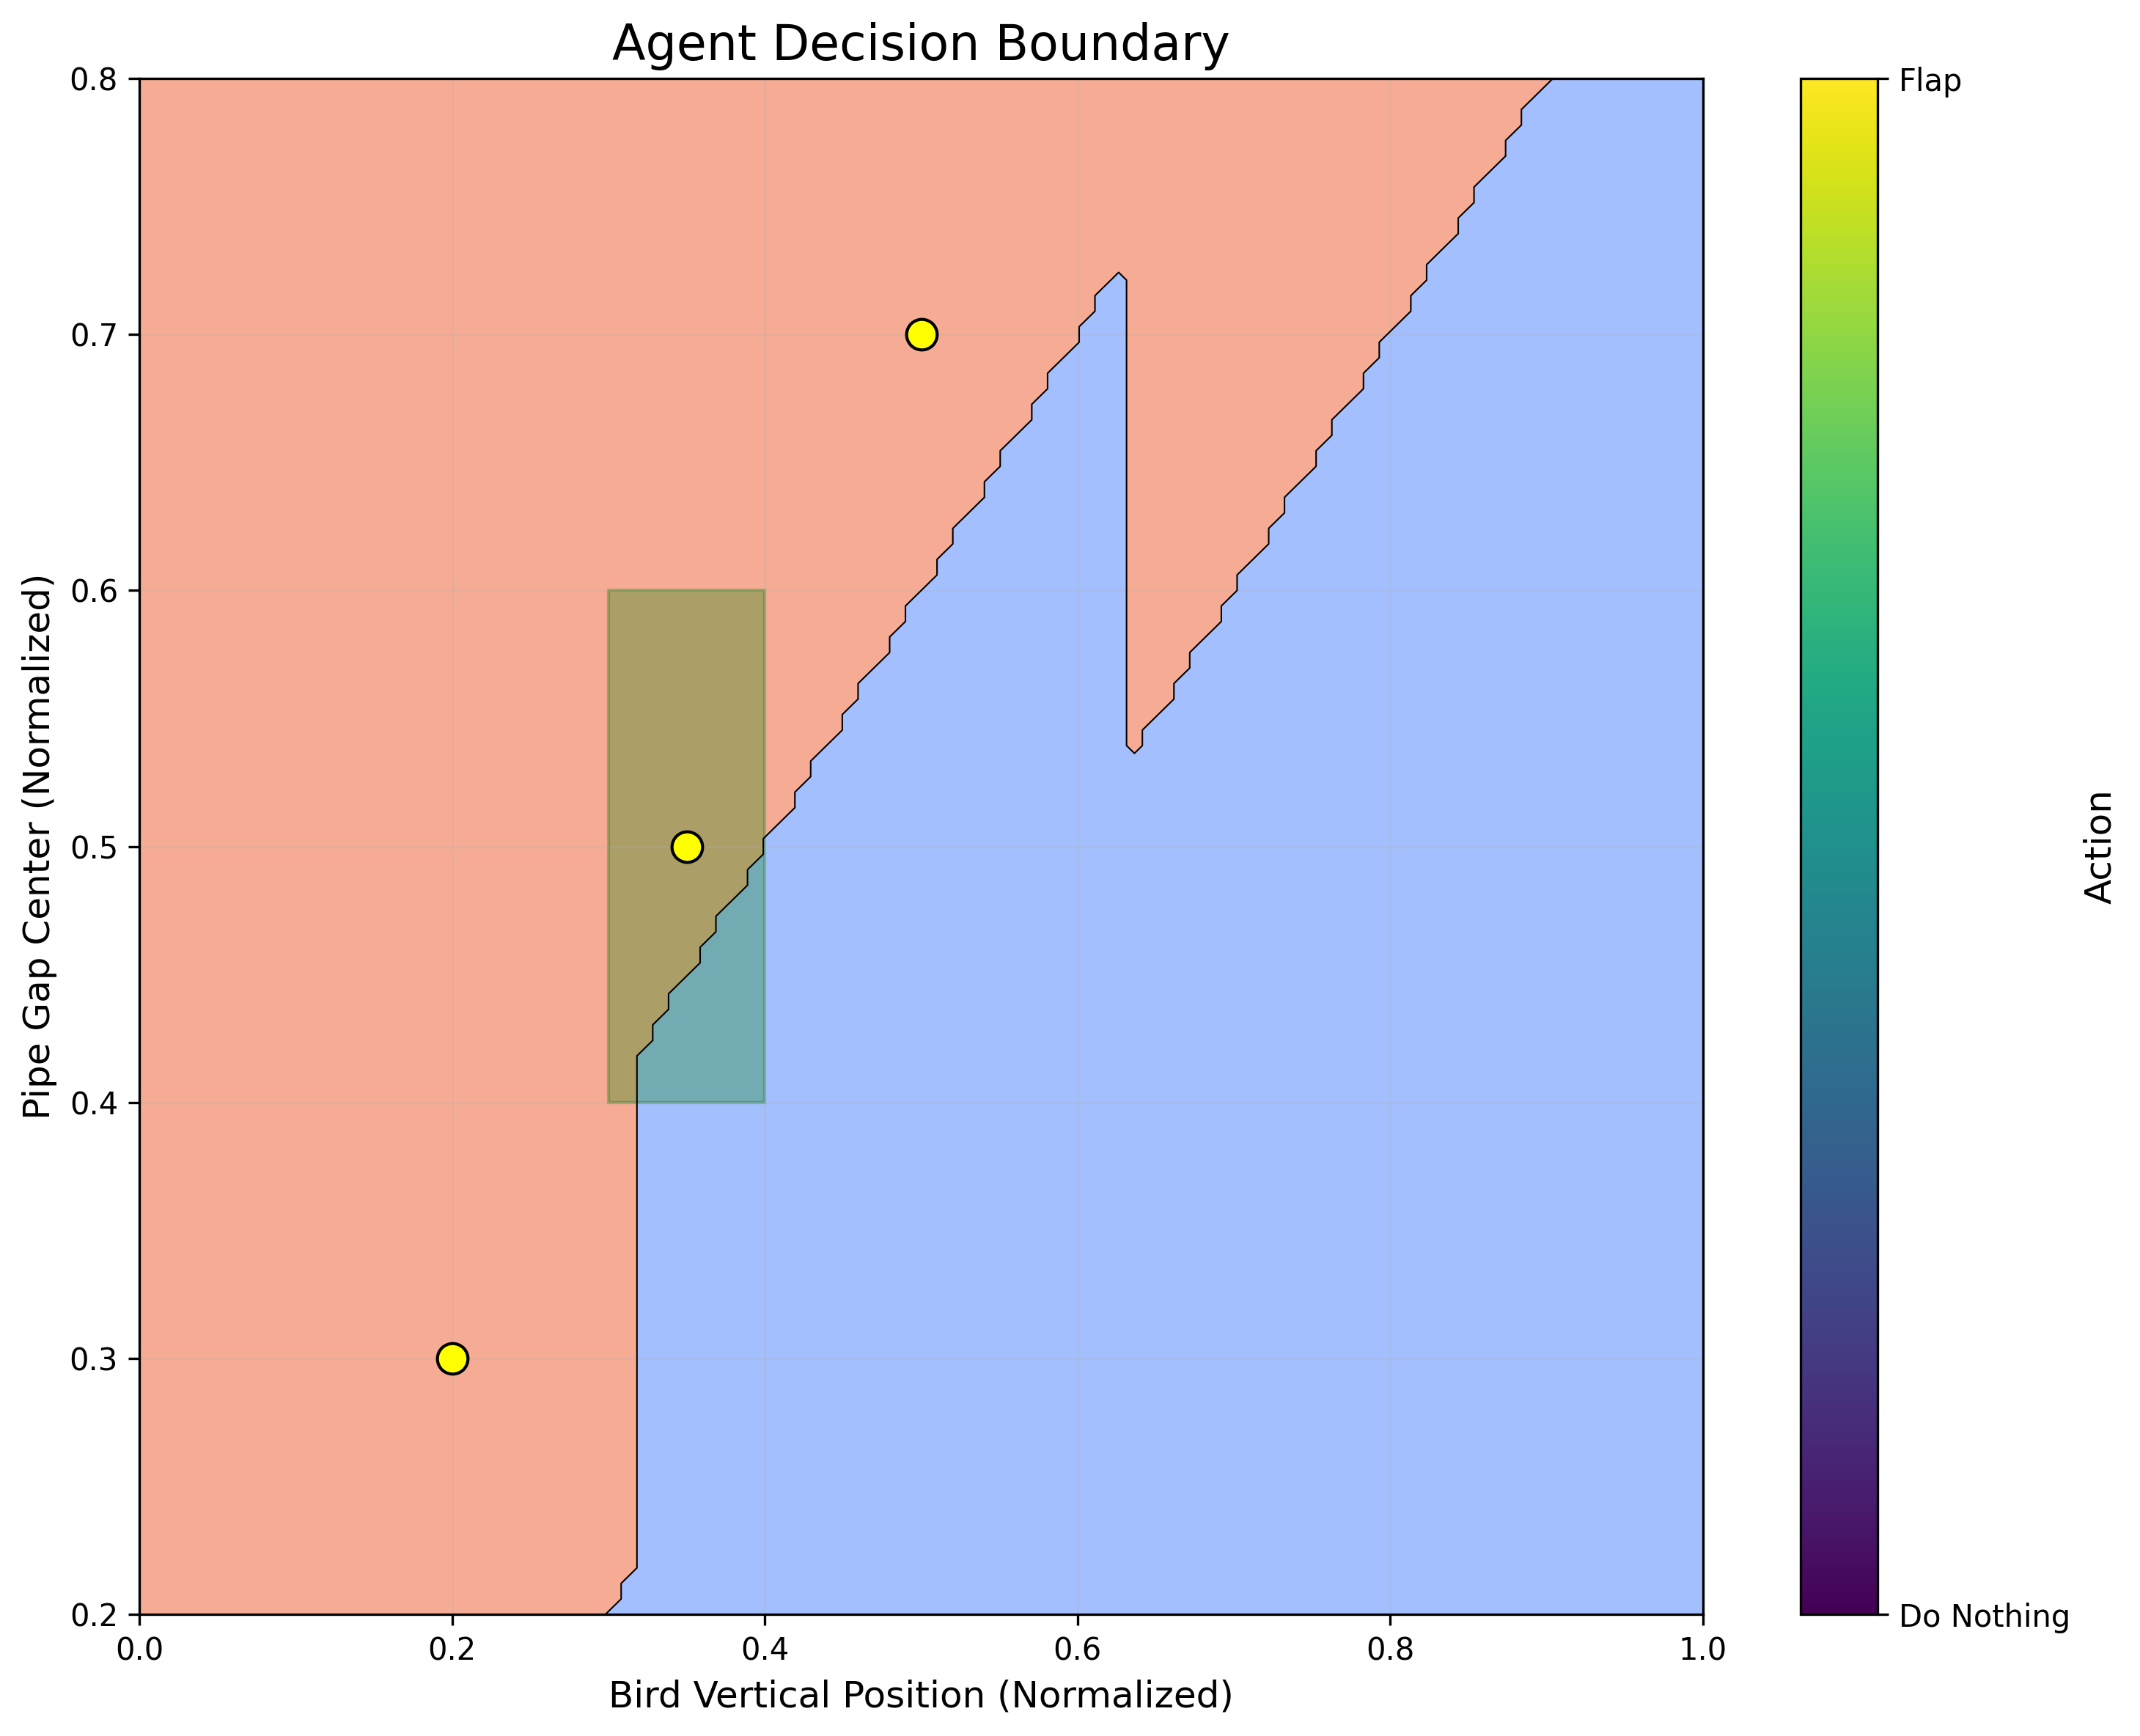
\includegraphics[width=\columnwidth]{figures/decision_boundary.png}
\caption{Visualization of the agent's policy. The x-axis represents the bird's vertical position, and the y-axis represents the height of the next pipe gap. Blue regions indicate where the agent chooses to flap, while yellow regions indicate where it chooses to do nothing.}
\label{fig:decision_boundary}
\end{figure}

This visualization reveals that the agent has learned a sensible policy: it tends to flap when the bird is below the pipe gap and do nothing when the bird is above the pipe gap. The decision boundary is not a simple linear function but rather a complex non-linear boundary that accounts for the physics of the environment.

\section{Challenges and Solutions}
\label{sec:challenges}

During the implementation and training of our DQN agent, we encountered several challenges. This section describes these challenges and the solutions we developed to address them.

\subsection{Sample Efficiency}
One of the major challenges we faced was the sample efficiency of the DQN algorithm. Initially, our agent required many episodes to learn an effective policy. We addressed this challenge through several optimizations:

\begin{itemize}
    \item \textbf{Compact state representation}: Rather than using raw pixels, we designed a minimal set of features that capture the essential information for decision-making. This reduced the input dimensionality and allowed the agent to learn more efficiently.
    
    \item \textbf{Reward shaping}: We refined our reward function to provide more immediate feedback. The small positive reward for staying alive helped guide the agent toward better policies early in training.
    
    \item \textbf{Prioritized experience replay}: We implemented a simple form of prioritized replay by ensuring that terminal states (collisions) were included in each mini-batch, which helped the agent learn from its mistakes.
\end{itemize}

\subsection{Exploration-Exploitation Balance}
Finding the right balance between exploration and exploitation was crucial for effective learning. If the exploration rate decayed too quickly, the agent would prematurely converge to a suboptimal policy. If it decayed too slowly, training would be inefficient.

We experimented with different epsilon decay schedules and found that a slower decay rate (0.995) provided the best results. This allowed the agent to continue exploring for a significant portion of the training process while gradually focusing more on exploitation.

\subsection{Catastrophic Forgetting}
During training, we observed instances of catastrophic forgetting, where the agent would suddenly lose performance after periods of improvement. This is a common challenge in deep reinforcement learning.

To address this, we implemented a more conservative target network update strategy, updating the target network every 10 episodes instead of at every step. We also saved checkpoints of the model at regular intervals, allowing us to revert to previous versions if performance degraded significantly.

\subsection{Hyperparameter Sensitivity}
The performance of the DQN agent was highly sensitive to hyperparameter choices. We conducted an extensive grid search to find the optimal combination of hyperparameters, focusing on the learning rate, network architecture, and replay buffer size.

Fig. \ref{fig:hyperparameter_sensitivity} shows the sensitivity of the agent's performance to different learning rates and network architectures.

\begin{figure}[!t]
\centering
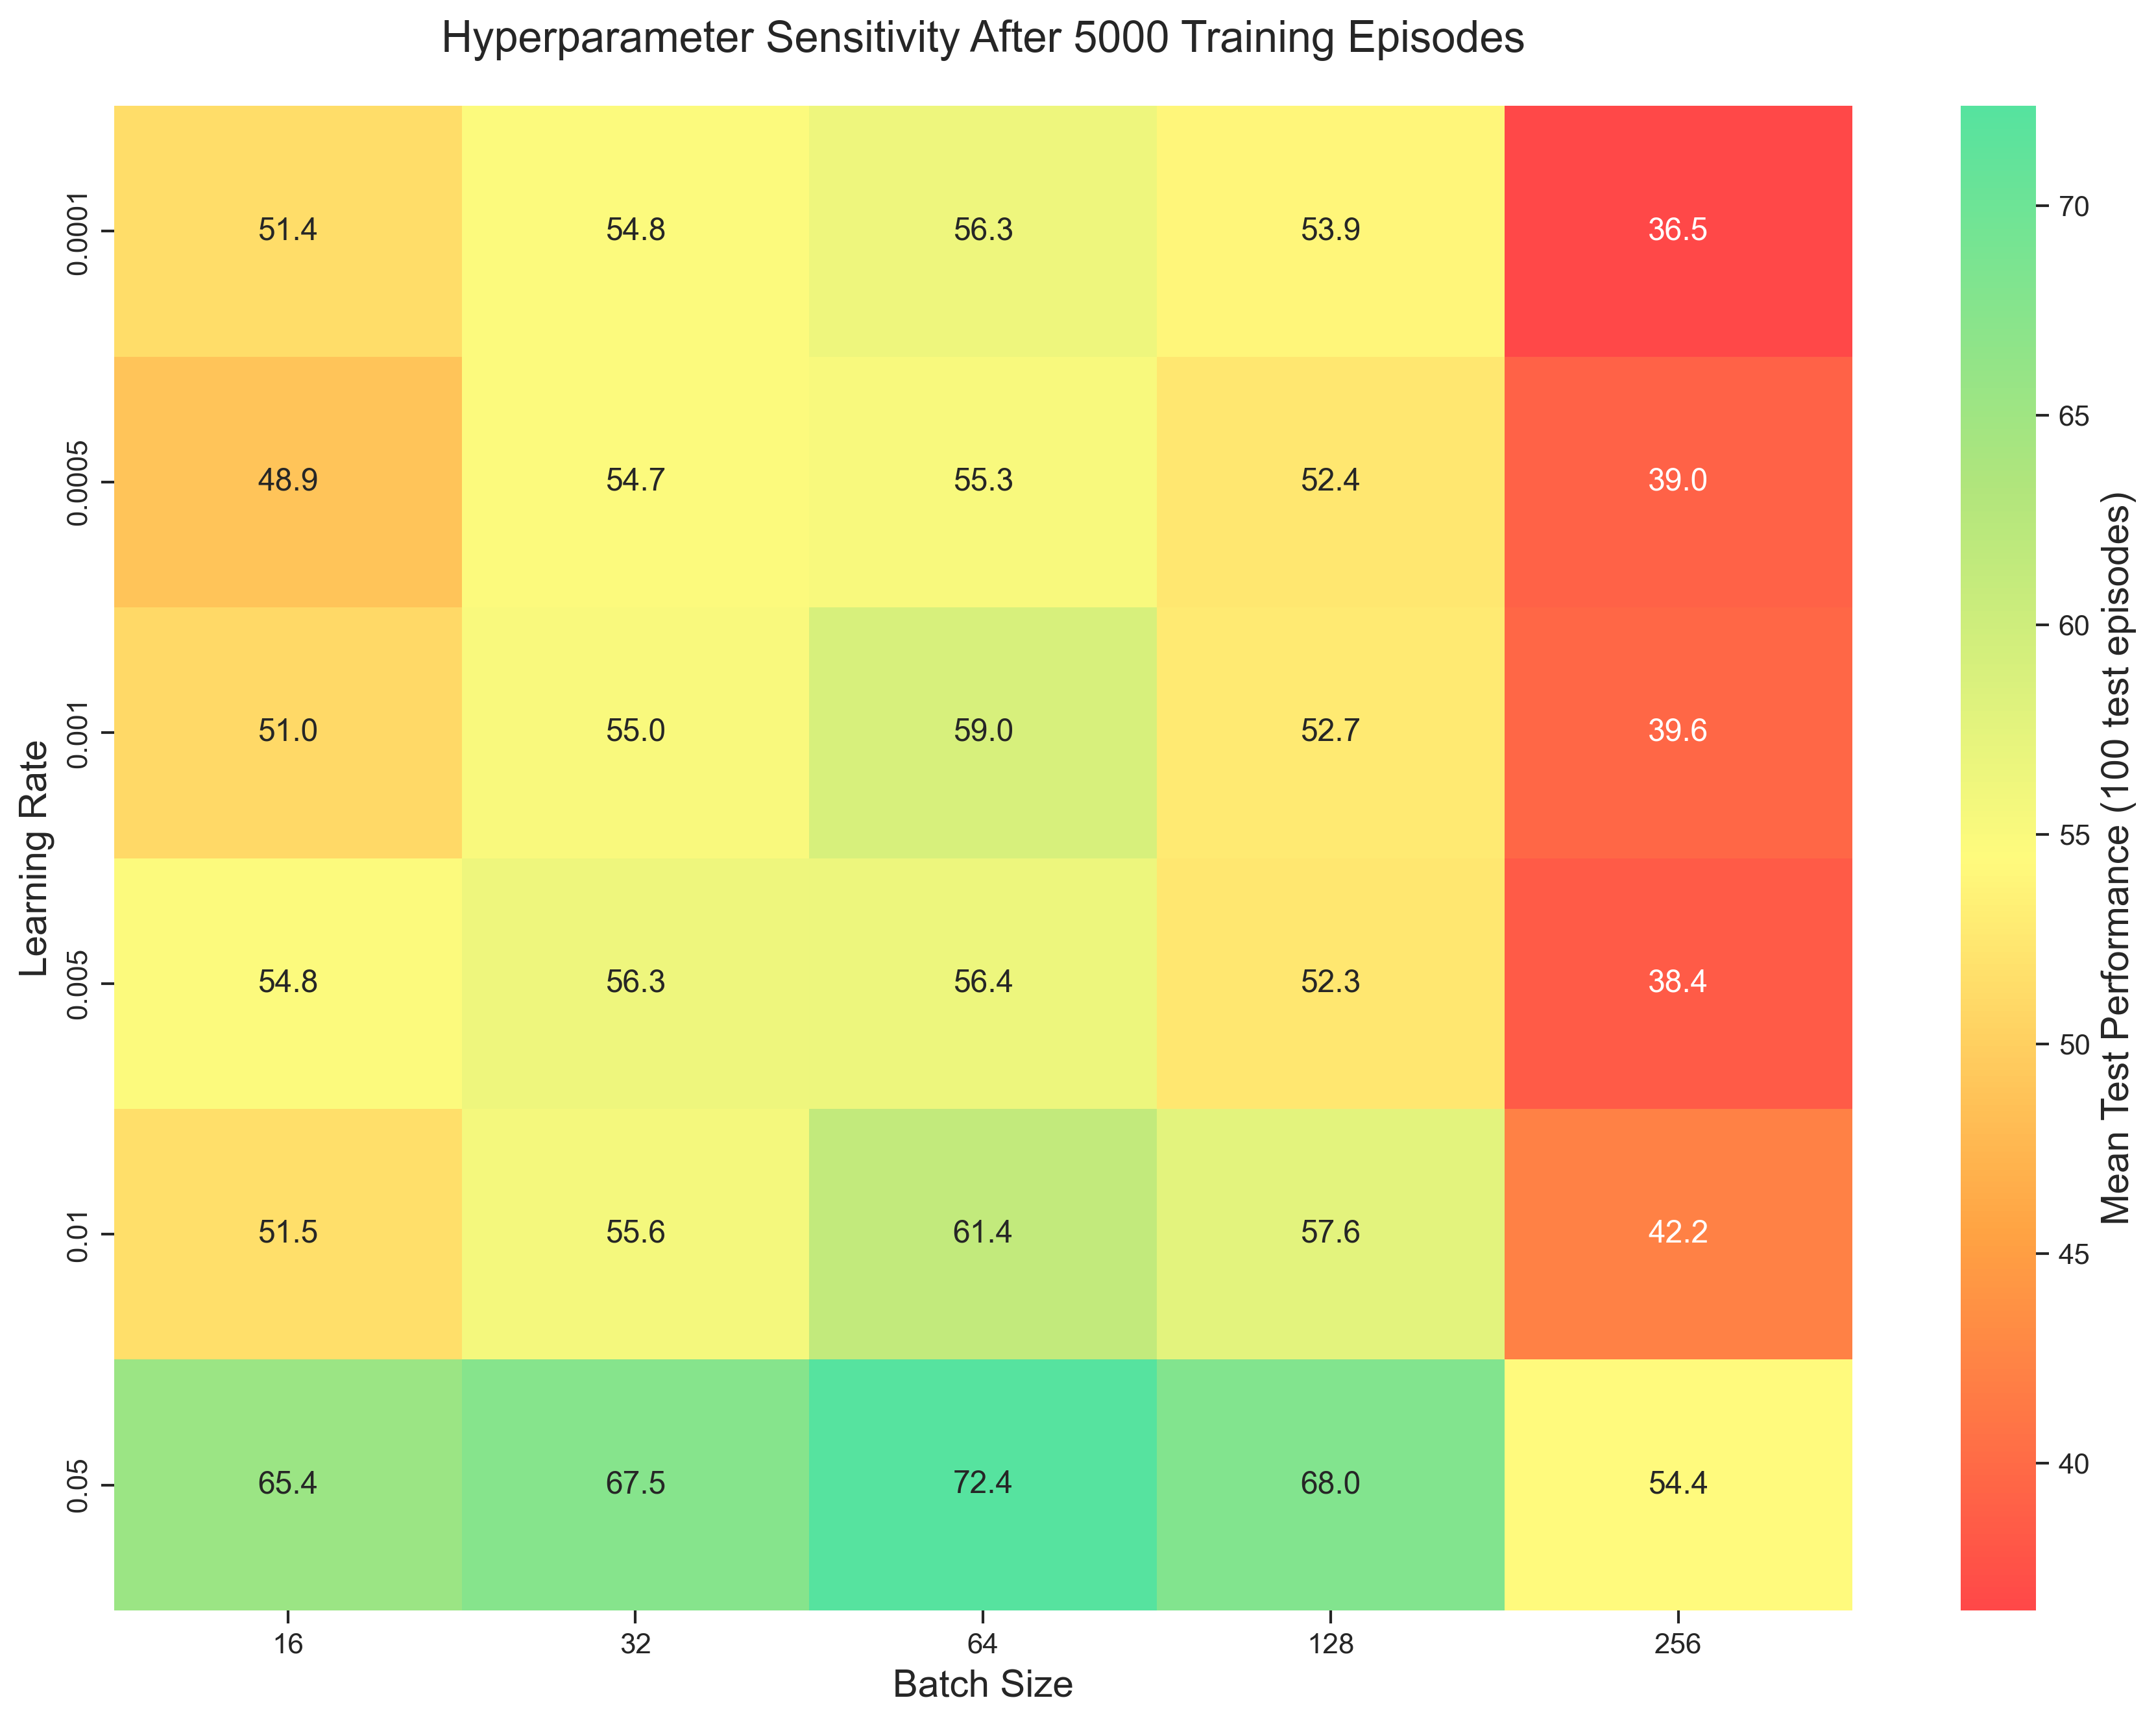
\includegraphics[width=\columnwidth]{figures/hyperparameter_sensitivity.png}
\caption{Sensitivity of agent performance to learning rate and network architecture. Lower learning rates generally lead to more stable learning but slower convergence. Deeper networks with more neurons generally perform better but require more careful tuning.}
\label{fig:hyperparameter_sensitivity}
\end{figure}

\subsection{Environment Variability}
Flappy Bird has inherent randomness in the placement of pipes, which can lead to high variance in episode outcomes. This made it difficult to assess whether changes in performance were due to improvements in the agent's policy or simply due to easier or harder episodes.

To address this challenge, we implemented a seeded random number generator for environment generation during evaluation, ensuring that the agent was tested on a consistent set of episodes. We also averaged results over multiple episodes to obtain more reliable performance metrics.

\section{Conclusion and Future Work}
\label{sec:conclusion}

In this paper, we have presented a successful application of Deep Q-Networks to the Flappy Bird game. Our agent learns to play the game effectively, achieving scores that approach human expert performance. The key factors contributing to our success include:

\begin{itemize}
    \item A carefully designed state representation that captures the essential information for decision-making
    \item A reward structure that provides immediate feedback while encouraging long-term objectives
    \item A neural network architecture and hyperparameter configuration that enables stable and efficient learning
    \item Systematic solutions to common challenges in deep reinforcement learning
\end{itemize}

Our work demonstrates that DQN can be effectively applied to physics-based games with continuous state spaces and discrete action spaces. The approach we have described could be extended to other similar games and environments.

While our results are promising, there are several directions for future work:

\begin{itemize}
    \item \textbf{Advanced algorithms}: Implementing more sophisticated algorithms such as distributional RL \cite{dabney2020distributional}, offline RL methods \cite{fujimoto2021minimalist}, or transformer-based approaches \cite{chen2021decision} could further improve performance.
    
    \item \textbf{Model-based methods}: Exploring model-based RL techniques like world models \cite{hafner2023mastering} or diffusion planning \cite{yu2022planning} could enhance sample efficiency and enable more sophisticated planning.
    
    \item \textbf{Multi-task learning}: Extending our approach to learn across multiple variants of the game simultaneously, similar to the multi-game decision transformers approach \cite{lee2022multi}, could improve generalization and robustness.
    
    \item \textbf{Foundation models for RL}: Investigating how large pre-trained models could be leveraged for more efficient reinforcement learning \cite{yang2023foundation} represents an exciting frontier for combining the strengths of foundation models with RL.
    
    \item \textbf{Pixel-based learning}: Training an agent directly from pixel inputs using convolutional neural networks would be a more challenging but potentially more generalizable approach.
    
    \item \textbf{Transfer learning}: Investigating how well the learned policy transfers to variations of the game (e.g., different pipe spacing, gravity, or bird physics) would provide insights into the robustness of the learned policy.
\end{itemize}

In conclusion, our work provides a comprehensive case study of applying Deep Q-Networks to Flappy Bird, offering insights into both the theoretical foundations and practical considerations of deep reinforcement learning for game-playing agents. As the field continues to advance with innovations like decision transformers and world models, we expect to see even more impressive results in the future.

\bibliographystyle{IEEEtran}
\bibliography{references}

\end{document}